\chapter{Introduction}
\section{EMG}
The rapid growth of wearable technology and the increasing availability of electromyography (\textbf{EMG}) wrist devices have opened up new possibilities for monitoring and analyzing human movements. \\

\subsection{The putEMG Dataset}
The putEMG dataset \cite{Kaczmarek2019PutEMGADataset} contains multi-channel surface electromyographic activity recorded from forearm. 
\subsubsection{Experiment Procedures}
Experiments were originally conducted on 44 participants. At each session the participant wore a 24 (8x3) electrode matrix and performed a series of 7 different actions separated by an idle state:
\begin{itemize}
    \item 0 - Idle state
    \item 1 - Fist
    \item 2 - Flexion
    \item 3 - Extension
    \item 6 - Pinch index
    \item 7 - Pinch middle
    \item 8 - Pinch ring
    \item 9 - Pinch small
\end{itemize}

\textit{Action Block} - The basic experiment procedure. A series of gestures and idle states performed as follows:\\

\textbf{for} $i$ in \textit{action\_set}:
\begin{enumerate}
    \item  \textbf{Do} gesture $i$ for $1$ or $3$ seconds (depending on trajectory - more on this later)
    \item   \textbf{Do} idle gesture for $3$ seconds
\end{enumerate}
 Between action blocks user were able to relax and move their hands freely for 10 seconds. A relax period is marked as -1. Each action block begins and ends with an idle gesture.

\textit{Trajectory} - A series of action blocks separated by relax periods.\\
Trajectory Types - 
\begin{itemize}
    \item \textit{repeats\_long} - 7 action blocks, each block contains 8 repetitions of each active gesture: [relax] 0-1-0-1-0-1-0-1-0-1-0-1-0-1-0-1-0 [relax] 0-2-0-2-0-2-0-2-0-2-0-2-0-2-0-2-0 [relax] 0-3-0... ,
    \item \textit{sequential} - 6 action blocks, each block is a subsequent execution of all active gestures: [relax] 0-1-0-2-0-3-0-6-0-7-0-8-0-9-0 [relax] 0-1-0-2-0-3-0-6-0-7-0-8-0-9-0 [relax] 0-1-0-2-0... ,
    \item \textit{repeats\_short} - 7 action blocks, each block contains 6 repetitions of each active gesture: [relax] 0-1-0-1-0-1-0-1-0-1-0-1-0 [relax] 0-2-0-2-0-2-0-2-0-2-0-2-0 [relax] 0-3-0... .
\end{itemize}
In a single experiment session a user performed the 3 trajectory types once which is summed to repeat each gesture 20 times.

Each participant had 2 sessions separated by minimum one week.

\subsection{Dataset Structure}
The dataset contains a csv file per user experiments (44 users X 2 Experiment sessions X 3 trajectory types = 264 files).
Each csv file contains a data frame with the following columns:
\begin{itemize}
    \item 24 EMG\_$i$ columns (1 per electrode) - The raw ADC signal value. A raw ADC signal read can be converted to milivolot using the following formula:
    $$N \rightarrow \frac{N \cdot 5}{2^{12}}\frac{1000}{200}[mV]$$
    \item TRAJ\_1- The gesture that was presented to the participant
    \item TRAJ\_GT\_NO\_FILTER - Gesture labeling using video stream gesture recognition algorithm. A VGGNet based recognition with no filter.
    \item TRAJ\_GT - The output of the median filter applied to the VGGNet and a window of 250 ms before presenting the action $i$ to 2000 ms after presenting the next action where outside this window action $i$ was discarded. \\ \textit{This column values were taken as ground true for the purpose of this research.}
    
\end{itemize}
% The putEMG dataset \cite{Kaczmarek2019PutEMGADataset} comprises multi-channel surface electromyographic (EMG) activity recorded from the forearm. The experimental device is equipped with 24 electrodes arranged in three rows of eight electrodes around the wrist. Participants execute a predefined sequence of gestures at a specific tempo. Each participant repeats this sequence two weeks after their initial performance.\\

% \textit{Action Block} - The basic experiment procedure. A series of gestures and idle states performed as follows:\\

%         \textbf{for} $i$ in \textit{action\_set}:
%         \begin{enumerate}
%             \item  \textbf{Do} gesture $i$ for $1$ or $3$ seconds (depending on trajectory - more on this later)
%             \item   \textbf{Do} idle gesture for $3$ seconds
%         \end{enumerate}
%          Between action blocks user were able to relax and move their hands freely for 10 seconds. A relax period is marked as -1. Each action block begins and ends with an idle gesture.
% Trajectory Types - 
%         \begin{itemize}
%             \item \textit{repeats\_long} - 7 action blocks, each block contains 8 repetitions of each active gesture: [relax] 0-1-0-1-0-1-0-1-0-1-0-1-0-1-0-1-0 [relax] 0-2-0-2-0-2-0-2-0-2-0-2-0-2-0-2-0 [relax] 0-3-0... ,
%             \item \textit{sequential} - 6 action blocks, each block is a subsequent execution of all active gestures: [relax] 0-1-0-2-0-3-0-6-0-7-0-8-0-9-0 [relax] 0-1-0-2-0-3-0-6-0-7-0-8-0-9-0 [relax] 0-1-0-2-0... ,
%             \item \textit{repeats\_short} - 7 action blocks, each block contains 6 repetitions of each active gesture: [relax] 0-1-0-1-0-1-0-1-0-1-0-1-0 [relax] 0-2-0-2-0-2-0-2-0-2-0-2-0 [relax] 0-3-0... .
%         \end{itemize}
%         In a single experiment session a user performed the 3 trajectory types once which is summed to repeat each gesture 20 times.
        
%         Each participant had 2 sessions separated by minimum one week.

% The dataset contains a csv file per user experiments (44 users X 2 Experiment sessions X 3 trajectory types = 264 files).
% Each csv file contains a data frame with the following columns:
% \begin{itemize}
%     \item 24 EMG\_$i$ columns (1 per electrode) - The raw ADC signal value. A raw ADC signal read can be converted to milivolt using the following formula:
%     $$N \rightarrow \frac{N \cdot 5}{2^{12}}\frac{1000}{200}[mV]$$
%     % \item TRAJ\_1- The gesture that was presented to the participant
%     % \item TRAJ\_GT\_NO\_FILTER - Gesture labeling using video stream gesture recognition algorithm. A VGGNet based recognition with no filter.
%     \item TRAJ\_GT - The output of the median filter applied to the VGGNet and a window of 250 ms before presenting the action $i$ to 2000 ms after presenting the next action where outside this window action $i$ was discarded. \\ \textit{This column values were taken as ground true for the purpose of this research.}
% \end{itemize}

\section{The Privacy Problem}

The EMG data collected from wrist devices contains personal information about users' hand movements, gestures, and muscle activity. This sensitive data could be exploited by malicious hackers with the intent to harm users or steal their identity. \\

Moreover, the increasing adoption of EMG data in various applications, such as rehabilitation, virtual reality, and human-computer interaction, highlights the need for accurate models. Accurate models need a large amount of data to be learned \\

EMG data must be safeguarded for privacy reasons, whereas EMG models require a substantial amount of data for effective training. These two objectives are not inherently aligned. \\



The objective of this thesis proposal is to learn a machine learning model of EMG data in a federated manner such that differential privacy is kept and accuracy is as good as we can get. By preserving the privacy of individual users while enabling robust analysis, we aim to strike a balance between privacy preservation and data utility. Additionally, we propose a novel approach that involves leveraging public users to embed gradients onto their subspace, further enhancing the privacy guarantees.\\

% start with EMG
% privacy problem 
% weak privacy - fl
% strong privacy - dp but degrades perf
% we search for a way to improve perf
% suggest use public users - use minimum public users and use for private users
\section{Weak Privacy and Strong Privacy}
Learning a gesture classifier in a \textbf{Federated} manner makes use of large population data while not pulling personal sensitive data from the wearable device. Moreover, federated learning has the advantage of personalizing model inference to a specific user. \\

But as demonstrated in the Netflix Prize competition, a renowned competition in the field of recommendation systems, \textbf{data anonymization does not ensure privacy}. While the contest aimed to improve movie recommendations by encouraging data sharing and algorithm development, it inadvertently exposed the potential risks of de-anonymization when researchers were able to de-anonymize users' personal data by cross referencing models trained on Netflix anonymized data with the IMDb dataset which is not anonymized. This event demonstrated how seemingly anonymized data can be de-anonymized when combined with additional information. 

A proposed technique to address this concern is \textbf{Differential privacy} \cite{Dwork2013ThePrivacy}. \\
Differential privacy offers a rigorous framework for privacy preservation in data analysis while still allowing valuable insights to be derived from the data. By introducing carefully calibrated noise into the computation process, it ensures that individual data points - in our case individual users -  remain indistinguishable in the final analysis results. This statistical privacy concept provides a formal and provable guarantee of privacy, even when an adversary has access to auxiliary information.\\

The \textbf{DP-SGD} \cite{Abadi2016DeepPrivacy} method is an efficient way to incorporate differential privacy to deep learning model. DP-SGD adds noise to the gradients before gradients are backpropagetd through the network. Moreover, DP-SGD computes the amount of privacy spent at each learning step and at the overall learning process. 

The \textbf{GEP} \cite{Yu2021DoLearning} proposes a method for estimating model gradients during training by incorporating them into a lower-rank subspace. Subsequently, privacy noise is introduced to the incorporated gradients. The motivation is that less noise is needed for the same amount of privacy. \\

\section{Our Contribution - Performance of Differential Private Federated Learning U sing Public Users }
Although effective, DP-SGD and GEP still exhibit a reduction in performance. To enhance the performance of EMG data models inference while maintaining privacy assurances, we propose a novel approach that relies on the participation of \textbf{public users} who are willing to expose their data. The public users' data is used for gradient subspace computation that all private gradients will be embedded into. We assume that the more gradients' "energy" is concentrated in the embedding subspace, the learned model will perform better.\\



% The proposed thesis aims to address the critical need for privacy in the analysis of EMG wrist data while preserving data utility. By leveraging differential privacy techniques and incorporating public users for gradient embedding, we strive to achieve robust privacy guarantees and enhance the accuracy of models trained on EMG data. This research has the potential to advance the field of privacy-preserving federated learning in the domain of EMG wrist data analysis and contribute to the development of secure and privacy-conscious wearable technologies.

% \begin{refsection} %% This is needed to create a separate references section for this chapter.
% \begingroup
% % increase max. interqword space so we don't get so many overfull hboxes due to unhyphenatable verbatim
% \spaceskip 3.33pt plus 6pt minus 1.11pt
% \chapter{Introduction}
% \label{sec: introduction}

% %% The following annotation is customary for chapter which have already been
% %% published as a paper.
% \blfootnote{Parts of this chapter have been published in Annalen der Physik \textbf{324}, 289 (1906) \cite{Einstein1906}.}

% %% It is only necessary to list the authors if multiple people contributed
% %% significantly to the chapter.
% \authors{Albert {\titleshape Einstein}}

% %% The '0pt' option ensures that no extra vertical space follows this epigraph,
% %% since there is another epigraph after it.
% \epigraph[0pt]{
%     Nature and nature's laws lay hid in the night; \\
%     God said `Let Newton be!' and all was light.
% }{Alexander Pope}

% \epigraph{
%     It did not last: the devil shouting `Ho. \\
%     Let Einstein be!' restore the status quo.
% }{Sir John Collings Squire}

% \begin{abstract}
% Lorem ipsum dolor sit amet, consectetur adipisicing elit, sed do eiusmod tempor incididunt ut labore et dolore magna aliqua. Ut enim ad minim veniam, quis nostrud exercitation ullamco laboris nisi ut aliquip ex ea commodo consequat. Duis aute irure dolor in reprehenderit in voluptate velit esse cillum dolore eu fugiat nulla pariatur. Excepteur sint occaecat cupidatat non proident, sunt in culpa qui officia deserunt mollit anim id est laborum.
% \end{abstract}

% %% Start the actual chapter on a new page.
% \newpage

% This document is intended to be both an example of the TU Delft dissertation template for \LaTeX, as well as a short introduction to its use. It is not intended to be a general introduction to \LaTeX{} itself,\footnote{We recommend \url{http://en.wikibooks.org/wiki/LaTeX} as a reference and a starting point for new users.} and we will assume the reader to be familiar with the basics of creating and compiling documents.

% Instructions on how to use this template under Windows and Linux, and which \LaTeX{} packages are required, can be found in \texttt{README.txt}.

% \section{Document Structure}
% \dropcap S{ince} a dissertation is a substantial document, it is convenient to break it up into smaller pieces. In this template we therefore give every chapter its own file. The chapters (and appendices) are gathered together in \texttt{dissertation.tex}, which is the master file describing the overall structure of the document.

% \mbox{\texttt{dissertation.tex}} starts with the line

% %% We need an empty line before the quote environment to work around a bug in
% %% the lettrine package, from which the drop command is derived.
% \begin{quote}
% \verb|\documentclass{_style/dissertation}|
% \end{quote}
% which loads the dissertation template. The template is based on the \LaTeX{} \texttt{book} document class and stored in \texttt{dissertation.cls}. The document class accepts several comma-separated options. By default, hyperlinks are shown in cyan, which is convenient when reading the dissertation on a computer, but can be expensive when printing. They can be turned black with the \texttt{print} option. This will also turn the headers dark gray instead of cyan. Moreover, it will add a 3~mm bleed around the page including crop marks. This will help the printer with the thumb indices, since they run right up to the page borders. Finally, the \texttt{fourier} option can be used to override the automatic font selection (see below).

% A dissertation is a big document, which makes it easy to miss warnings about the layout in the \LaTeX{} output. In order to locate problem areas, add the \texttt{draft} option to the \verb|\documentclass| line. This will display a vertical bar in the margins next to the paragraphs that require attention.

% The contents of the dissertation are included between the \verb|\begin|\allowbreak\verb|{document}| and \verb|\end{document}| commands, and split into three parts by
% \begin{enumerate}
% \item\verb|\frontmatter|, which uses Roman numerals for the page numbers and is used for the title page and the table of contents;
% \item\verb|\mainmatter|, which uses Arabic numerals for the page numbers and is the style for the chapters;
% \item\verb|\appendix|, which uses letters for the chapter numbers, starting with `A'.
% \end{enumerate}
% The title page is defined in \texttt{title.tex} in the \texttt{title} folder and included verbatim with \verb|\begin{titlepage}

    % \begin{center}

    %     %% Extra whitespace at the top.
    %     \vspace*{2\bigskipamount}

    %     %% Print the title.
    %     {\makeatletter
    %         \titlestyle\bfseries\LARGE\@title
    %         \makeatother}

    %     %% Print the optional subtitle.
    %     {\makeatletter
    %         \ifx\@subtitle\undefined\else
    %             \bigskip
    %             \titlefont\titleshape\Large\@subtitle
    %         \fi
    %         \makeatother}

    % \end{center}

    % \cleardoublepage
    % \thispagestyle{empty}

    \begin{center}

        %% The following lines repeat the previous page exactly.

        \vspace*{2\bigskipamount}

        %% Print the title.

        {\makeatletter
            \titlestyle\bfseries\LARGE Bar-Ilan University \\
            The Faculty of Engineering \\
            \bigskip
            Electrical Engineering, Data Science Track \\
            \bigskip
            MSc. Research Proposal
            \makeatother}
        \bigskip
        \bigskip
        \bigskip

    \end{center} 
      \textbf{Research Subject:} 
     \begin{center}
         
        
        \bigskip
        {\makeatletter
            \titlestyle\bfseries\LARGE 
            \@title
            \makeatother}

        %% Print the optional subtitle.
        {\makeatletter
            \ifx\@subtitle\undefined\else
                \bigskip
                \titlefont\titleshape\Large\@subtitle
            \fi
            \makeatother}

        %% Uncomment the following lines to insert a vertically centered picture into
        %% the title page.
        %\vfill
        %\includegraphics{title}
        \vfill

        %% Apart from the names and dates, the following text is dictated by the
        %% promotieregelement.

        % {\Large\titlefont\bfseries MSc Research Proposal}


        % for the purpose of obtaining the degree of \\
        % MSc in Electrical Engineering - Data Science Track

        % at The \textit{Alexander Kofkin} Faculty of Engineering, \textit{Bar-Ilan} University

        % by the authority of the Rector Magnificus, prof.~dr.~ir.~T.H.J.J.~van der Hagen,

        % chair of the Board for Doctorates

        % to be defended publicly on

        %     [date= weekday (word) day (number), month (word) year (number)] at [hh:mm (number)] o'clock

        % \bigskip
        % \bigskip

        by
        
        \bigskip

        %% Print the full name of the author.
        \makeatletter
        {\Large\titlefont\bfseries\@firstnames\ {\Large\titlefont\bfseries\@lastname}} \\
        \bigskip
        Supervisor: 
        {\Large\titlefont\bfseries Dr. Ethan  {\Large\titlefont\bfseries Fetaya}}
        \makeatother

        \bigskip
        \bigskip

        % [highest academic title, name university, country]

        % born in [town/city, country of birth]

        %% Extra whitespace at the bottom.
        \vspace*{2\bigskipamount}

    \end{center}

    % \clearpage
    % \thispagestyle{empty}

    %% The following line is dictated by the promotieregelement.
    % \noindent This dissertation has been approved by the promotors.

    % \bigskip
    % \noindent Composition of the doctoral committee:
    %% List the committee members, starting with the Rector Magnificus and the
    %% promotor(s) and ending with the reserve members.
    % \begin{tabbing}
    %     \hspace{\tabcolsep}\=\hspace{0.33\textwidth}\=\hspace{0.66\textwidth}                   \\[-3\medskipamount]
    %     \> Rector Magnificus,          \> chairperson\\
    %     \> Prof.\ dr.\ A.\ Kleiner,    \> Delft University of Technology, \textit{promotor}      \\
    %     \> Dr.\ A.A.\ Aaronson,        \> Delft University of Technology, \textit{copromotor}    \\[\medskipamount]
    %     \>\textit{Independent members:}                                                        \\[\smallskipamount]
    %     \>Prof.\ dr.\ A.\ Jansen       \> Delft University of Technology                         \\
    %     % Special case, only for very long names
    %     \>Prof.\ dr.\ ir.\ A.B.C.D.\ van de Lange-Achternaam                                    \\
    %     \>                             \> Delft University of Technology                         \\
    %     \>Prof.\ dr.\ N.\ Nescio       \> Politecnico di Milano, Italy                       \\
    %     \>Prof.\ dr.\ ir.\ J.\ Doe,    \> Delft University of Technology, reserve member             \\[\medskipamount]
    %     \>\textit{Other members:}                                                               \\[\smallskipamount]
    %     \>Prof.\ dr.\ ir.\ J.\ de Wit, \> Delft University of Technology                         \\
    %     \>Dr.\ ir.\ Q.\ de Zwart,      \> Delft University of Technology\\
    % \end{tabbing}

    %% Include the following disclaimer for committee members who have contributed
    %% to this dissertation. Its formulation is again dictated by the
    %% promotieregelement.
    % \medskip
    % \noindent Prof.\ dr.\ ir.\ J.\ de Wit of Delft University of Technology has contributed greatly to the preparation of this dissertation.

    %% Here you can include the logos of any institute that contributed financially
    %% to this dissertation.
    % \vfill
    % \begin{center}
    %     
\includegraphics[height=0.5in]{_logos/tudelft}
    %     \hspace{2em}
    %     
\includegraphics[height=0.5in]{_logos/casimir} \\
    %     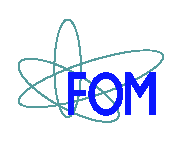
\includegraphics[height=0.5in]{_logos/fom}
    %     \hspace{2em}
    %     
\includegraphics[height=0.5in]{_logos/nwo}
    % \end{center}
    % \vfill

    % \noindent
    % \begin{tabular}{@{}p{0.2\textwidth}@{}p{0.8\textwidth}@{}}
    %     \textit{Keywords:}    & \ldots                                                                                        \\[\medskipamount]
    %     \textit{Printed by:}   & Johannes Gutenberg                                                                            \\[\medskipamount]
    %     \textit{Cover by:} & Beautiful cover art that captures the entire content of this thesis in a single illustration.
    % \end{tabular}

    % \vspace{4\bigskipamount}

    % \noindent Copyright \textcopyright{} \the\year{} by{
    %     \makeatletter
    %     \@initials~\@lastname
    %     \makeatother
    % }

    %% Uncomment the following lines if this dissertation is part of the Casimir PhD
    %% Series, or a similar research school.
    %\medskip
    %\noindent Casimir PhD Series, Delft-Leiden 2015-01

    % \medskip
    % \noindent ISBN 000-00-0000-000-0

    % \medskip
    % \noindent An electronic copy of this dissertation is available at\\
    % \url{https://repository.tudelft.nl/}.

\end{titlepage}

|,\footnote{Note that it is not necessary to specify the file extension.} (see below). Additionally, it is possible to include a preface, containing, for example, the acknowledgements. An example can be found in \texttt{preface.tex}. The table of contents is generated automatically with the \verb|\tableofcontents| command. Chapters are included after \verb|\mainmatter| and appendices after \verb|\appendix|. For example, \verb|\include{|\allowbreak\verb|introduction/|\allowbreak\verb|introduction}| includes \verb|introduction/introduction.tex|, which contains this introduction.

% \section{Title Page}

% \dropcap T{he} title pages are defined in \texttt{title/title.tex}, which you will have to modify according to your needs. Note that these pages are subject to the requirements of the \emph{promotieregelement} and cannot be changed at will. The title page may be written in the English or Dutch language
% preferably in the same language as the dissertation.
% Apart from the names and dates, most of the text is dictated literally.

% Since the thesis title and name of the author appear several times throughout the document (on the title page, but also in, \emph{e.g.}, the preface and cv), special commands are provided so they only have to be specified once. The title (and optional subtitle) can be specified with

% \begin{quote}
% \verb|\title[Optional subtitle]{Title}|
% \end{quote}
% The name of the author is specified with
% \begin{quote}
% \verb|\author{First name}{Last name}|
% \end{quote}
% Note that the first and last name are separate arguments, since they may be printed in different font shapes. The \verb|\title| and \verb|\author| commands also ensure that the title and author appear in the metadata of the final PDF.

% See \texttt{title/title.tex} for detailed documentation on the comment and layout of the title pages. Logos of institutes that have contributed financially to the dissertation may be included on reverse side of the title page. A few example logos can be found in the \verb|_logos| folder.

% \section{Chapters}

% \dropcap E{ach} chapter has its own file. For example, the \LaTeX{} source of this chapter can be found in \texttt{introduction/introduc\-tion\allowbreak.tex}. A chapter starts with the command

% \begin{quote}
% \verb|\chapter{Chapter title}|
% \end{quote}
% This starts a new page, prints the chapter number and title and adds a link in the table of contents. If the title is very long, it may be desirable to use a shorter version in the page headers and the table of contents. This can be achieved by specifying the short title in brackets:

% \begin{quote}
% \verb|\chapter[Short title]{Very| \verb|long| \verb|title| \verb|with| \verb|many| \verb|words| \verb|which| \verb|could| \verb|not| \verb|possibly| \verb|fit| \verb|on| \verb|one| \verb|line}|
% \end{quote}
% The command \verb|\frontmatter| sets page numbering to lower case Roman, and removes the chapter numbering. \verb|\mainmatter| sets both numberings to Arabic (`normal') numbers. \verb|\appendix| sets the chapter numbering to upper case Latin letters. \verb|\backmatter| removes the chapter numbering again.

% If (parts of) the chapter have already been published elsewhere, it is customary to add a reference. This can be done with the special unnumbered footnote command \verb|\blfootnote|. For example,

% \begin{quote}
% \verb|\blfootnote{Parts| \verb|of| \verb|this| \verb|chapter| \verb|have| \verb|been| \verb|published| \verb|in| \verb|Annalen| \verb|der| \verb|Physik| \verb|\textbf{324},| \verb|289| \verb|(1906)|\\\verb|\cite{Einstein1906}.}|
% \end{quote}
% generates the footnote at the beginning of this chapter. Because this footnote is unnumbered, the \texttt{hyperref} package may throw a warning, which safely be ignored.

% If multiple people have contributed significantly to this chapter, they can be lister with the \verb|\authors| command. This can be followed by a quotation using \verb|\epigraph| as shown above. Finally, it is customary for a dissertation to include an abstract for every chapter (except perhaps the introduction). This can be accomplished with the \texttt{abstract} environment. The abstract should be followed by \verb|\newpage| to start the chapter text on a new page.

% In a dissertation, each chapter has its own list of references. These can be generated with the special command \verb|\references|\allowbreak\verb|{dissertation}| from \texttt{disser\-tation.bib} at the end of the chapter. Note that this means that you need to run a command like \texttt{biber chapter-1/\allowbreak chapter-1} for each chapter. The template will automatically generate clickable hyperlinks if a URL or DOI (digital object identifier) is present for the reference. Although it is possible to manage the bibliography by hand, we  recommend using Zotero\footnote{Open source, desktop and online version available from \url{https://www.zotero.org}}, Mendeley\footnote{Desktop and online version available from \url{https://www.mendeley.com/}}, EndNote, or JabRef\footnote{Open source, specialised \texttt{*.bib} file editor; desktop only, available from \url{http://jabref.sourceforge.net/}}.

% Chapters are subdivided into sections, subsections, subsubsections, and, optionally, paragraphs and subparagraphs. All can have a title, but only sections and subsections are numbered. As with chapters, the numbering can be turned off by using \verb|\addsec{...}| instead of \verb|\section{...}|, and similarly for the subsection.
% \section{\textbackslash section\{\ldots\}}
% \subsection{\textbackslash subsection\{\ldots\}}
% \subsubsection{\textbackslash subsubsection\{\ldots\}}
% \paragraph{\textbackslash paragraph\{\ldots\}}
% Lorem ipsum dolor sit amet, consectetur adipisicing elit, sed do eiusmod tempor incididunt ut labore et dolore magna aliqua. Ut enim ad minim veniam, quis nostrud exercitation ullamco laboris nisi ut aliquip ex ea commodo consequat. Duis aute irure dolor in reprehenderit in voluptate velit esse cillum dolore eu fugiat nulla pariatur.
% \subparagraph{\textbackslash subparagraph\{\ldots\}}
% Excepteur sint occaecat cupidatat non proident, sunt in culpa qui officia deserunt mollit anim id est laborum.

% \section{Fonts and Colors}

% \dropcap T{he} fonts used by this template can be chosen via a documentclass option. If you leave the option (as given in the template) \verb|\documentclass|\allowbreak\verb|[fourier]|\allowbreak\verb|{_style/dissertation}|, Latex will use Utopia for titles and the main text, Fourier for math, and Latin Modern for sans-serif and monospaced text.
% If, on the other hand, you remove this option and use \verb|\documentclass|\allowbreak\verb|{_style/|\allowbreak\verb|dissertation}|,  you will get Roboto Slab for titles, Roboto (if you use PdfLatex) or Arial (if you use XeLatex or LuaLatex) for the main text, Courier New for monospace and Arev\footnote{A version of Bitstream Vera Sans with \LaTeX\ math support}for math.
% This is in line with the current Corporate style of the TU Delft.

% This template supports the use of drop caps, a large colored initial at the beginning of a chapter or section, via the \verb|\dropcap| command:

% \begin{quote}
% \verb|\dropcap{L}{orem} ipsum...|
% \end{quote}
% The first argument is the capital that will be printed on two lines (in the title color), and the second argument is the rest of the word. Depending on the font, the latter may be printed in small caps.

% The corporate colors of the TU Delft are cyan, black and white, available, respectively, via \verb|\textcolor{|\textcolor{tud primary}{\texttt{tud primary}}\verb|}{...}|, \verb|\textcolor|\allowbreak\texttt{\{\textcolor{black}{black}\}\{...\}} and \verb|\textcolor{|\allowbreak\texttt{white}\verb|}{...}|.
% Apart from these three, the house style defines the following basic colors, that can be used via \verb|\textcolor{tud |\textit{colorname}\verb|}{...}|:
% \begin{itemize}
%   \itemsep 0pt
%   \parskip 0pt
%   \item \textcolor{tud navy}{\textbf{navy}}
%   \item \textcolor{tud topaz}{\textbf{topaz}}
%   \item \textcolor{tud blue}{\textbf{blue}}
%   \item \textcolor{tud purple}{\textbf{purple}}
%   \item \textcolor{tud pink}{\textbf{pink}}
%   \item \textcolor{tud shiraz}{\textbf{shiraz}}
%   \item \textcolor{tud grapefruit}{\textbf{grapefruit}}
%   \item \textcolor{tud orange}{\textbf{orange}}
%   \item \textcolor{tud yellow}{\textbf{yellow}}
%   \item \textcolor{tud green}{\textbf{green}}
%   \item \textcolor{tud teal}{\textbf{teal}}
% \end{itemize}

% ISO~\num{80000} \cite{ISO80000} defines that in mathematical typesetting, only variables should be italised. This means that constants (numbers, units, functions such as \(\mathrm J_0, \sin\) etc.) and other text should be upright.
% A more accessible source for these typesetting rules is the SI brochure \cite[\S 2.3.1]{SIbrochure}. A few examples of correctly typeset math are shown below. The packages \texttt{siunitx} and \texttt{amsmath} (here loaded via \texttt{mathtools}) makes typesetting math correctly significantly easier.

% The rotational speed of the earth around the sun is approximately \(\varOmega_\text{earth} = 2 \uppi\,\si{rad.year^{-1}} \approx \SI{0.1991}{\micro\radian\per\second}\).\footnote{In \TeX, math mode is \emph{toggeled} using \texttt{\$...\$}, which is still what many people use. In \LaTeX, we can do this too, but we can also use a clear beginning and end of math mode, as \texttt{\textbackslash(...\textbackslash)}, which will make your code and possible error messages easier to understand.}

% The unnormalised sinc function is defined as follows:
% % in preamble: \DeclareMathOperator{\sinc}{sinc}
% \begin{equation}
%   \sinc x = \begin{cases}
%     0 & \text{where \(x = 0\)}\\
%     1 / \sin x & \text{else}
%   \end{cases}
% \end{equation}

% The following equation, commonly known as Euler's identity, consists of constants numbers only, and hence all symbols should be set upright:
% \begin{equation}
%   \mathrm e^{\mathrm i \uppi} + 1 = 0
% \end{equation}

% Here's a nice equation used as a demo by the \LaTeX\ font catalogue\footnote{\url{https://tug.org/FontCatalogue/}}
% \begin{equation}
%   \mathbfsf{B}(P)=\frac{\mu_0}{4\pi}\int\frac{\mathbfsf I \times \hat r ' }{r'^2} \mathrm dl
%     = \frac{\mu_0}{4\uppi}I\int\frac{\mathrm d\mathbfsf{l}\times\hat r'}{r'^2}
% \end{equation}

% \makeatletter
% \if@fourier
%   \section{Fourier}

The package \texttt{fourier} loads the Utopia font in \LaTeX. Use this informtion to your advantage when creating your figures \textthing.

\begin{itemize}
    \renewcommand\labelitemi\lefthand
    \item It has a more classical feel than the TU corporate style.
    \item It offers an upright \verb|\patial|: \(\partial\)
    \item It has some nice \floweroneleft\ ornaments \floweroneright
    \item It offers the official euro symbol \eurologo, which you may use instead of the default €, if you like.
\end{itemize}

\marginpar{\raggedright\caution this may be over the top.}
\definecolor{newred}{cmyk}{0,1,1,0.1}
\textcolor{newred}{\oldpilcrowfour}\,We few,
we happy few, we band of brothers; \textcolor{newred}
{\oldpilcrowfive}\,For he to-day that sheds his blood with
me \textcolor{newred}{\oldpilcrowsix}\,Shall be my brother;
be he ne'er so vile, \textcolor{newred}
{\oldpilcrowfour}\,This day shall gentle his condition.

% \else
%   \section{Roboto}

The TU Delft style prescribes Roboto Slab together with Arial.%
\footnote{\url{https://www.tudelft.nl/huisstijl/bouwstenen/typografie}}
Since Arial is not available in pdf\LaTeX, we will use regular Roboto instead.
Not surprisingly, this looks great together with Roboto Slab.

Roboto (Sans) has a dual nature. It has a mechanical skeleton
and the forms are largely geometric. At the same time,
the font features friendly and open curves. While some
grotesks distort their letterforms to force a rigid
rhythm, Roboto doesn't compromise, allowing letters to be
settled into their natural width. This makes for a more
natural reading rhythm more commonly found in humanist and
serif types.

Roboto Serif is designed to create a comfortable
and frictionless reading experience. Minimal and
highly functional, it is useful anywhere (even for app
interfaces) due to the extensive set of weights and widths
across a broad range of optical sizes. While it was
carefully crafted to work well in digital media, across
the full scope of sizes and resolutions we have today, it
is just as comfortable to read and work in print media.

Roboto has several styles of digits:
\begin{itemize}
    \item `Normal' lining numbers
    \begin{itemize}
        \item Proportional: \robotoLF{1234567890}
        \item Tabular: \robotoTLF{1234567890}
    \end{itemize}
    \item Ols style numbers
    \begin{itemize}
        \item Proportional: \robotoOsF{1234567890}
        \item Tabular: \robotoTOsF{1234567890}
    \end{itemize}
\end{itemize}

Furthermore, the font is available in many different weights:
\begin{itemize}
    \itemsep 0pt
    \parskip 0pt
    \item \robotoThin{robotoThin}
    \item \robotoLight{robotoLight}
    \item \robotoRegular{robotoRegular}     
    \item \robotoMedium{robotoMedium}      
    \item \robotoBold{robotoBold}
    \item \robotoBlack{robotoBlack}    
\end{itemize}

The documentation for the \LaTeX\ package can be found on ctan\footnote{\url{https://ctan.org/pkg/roboto}}; 
The original truetype fonts are available at google\footnote{\url{http://www.google.com/webfonts}}
and are licensed under the
Apache or OFL licenses; the texts may be found in the
doc directory. The opentype and type1 versions were created
using fontforge and cfftot1. The support files were created
using autoinst and are licensed under the terms of the LaTeX
Project Public License. The maintainer of this package is
Bob Tennent (rdt at cs.queensu.ca)

% \fi
% \makeatother

% % \printreferences
% \endgroup
% \end{refsection}
